
\chapter{An evolutionary perspective on epistasis and the missing heritability}
\label{Results1}
\lhead{Chapter 2. \emph{Epistasis under selection}}
\section{Abstract}

\setstretch{1}
While some studies have pointed out the failings of genome wide association studies for fitness traits, and thrown doubt upon the common disease-common variant paradigm, several others have nominated epistasis as a potential mechanism to reconcile these problems, and as a source of the `missing heritability'. This study sought to investigate these claims in the context of two-locus functional epistasis in traits under selection. A genetic algorithm was used to create two-locus genotype-phenotype maps that were optimised to maximise high additive variance sustained over long evolutionary periods. The deterministic expectations for allele frequency trajectories, genetic variance partitions, and detection power for different association strategies for these patterns and others were calculated. The impact of drift was also considered through stochastic simulations. Overall it was shown that while substantial genetic variance could be maintained at intermediate frequencies under selection, only a very small proportion of this was comprised of additive variance, diminishing the role of epistasis in the problem of `missing heritability'. Results from the power analysis were highly stratified, favouring one dimensional scans when linkage disequilibrium between causal variants and observed SNPs was low, and exhaustive pairwise scans when LD was high. Under the model of abundant epistasis contributing to complex fitness traits, the common disease-common variant hypothesis appears tenable. For fitness traits in particular, parameterising association studies to identify additive effects, even when the main purpose is to detect additive variance, is likely to be less powerful than parameterisations that include dominance, or strategies that expand the search to two dimensions to search for epistasis.

%In fitness traits in particular, epistasis may play an important role in maintaining genetic variation amongst common polymorphisms, thus contributing to the genetic variance for relatively prolonged periods. This could provide opportunities for finding otherwise undetectable small additive effects, by searching for epistatic interactions. Using a genetic algorithm to generate candidate epistatic patterns, as well as using already characterised epistatic patterns, simulations showed that while numerous types of epistatic patterns could maintain additive genetic variance at intermediate frequencies for much greater time scales than independent additive effects, these effects are small compared to non-additive components, diminishing the role of two-locus epistasis in the problem of missing heritability in fitness-related traits. Further, given this potential source of non-additive genetic variance, its detection is heavily dependent upon strong linkage disequilibrium between causal variants and observed SNPs, with the power of two-dimensional scans falling much more rapidly than one-dimensional scans as linkage disequilibrium decreases. Consequently, 


\section{Introduction}
\setstretch{1.6}

Our understanding of the mechanisms behind complex traits is gradually improving with the widespread use of genome wide association studies (GWASs), through the identification of putative causative genes \citep{Hindorff2010}. However this type of analysis has thus far only uncovered a small fraction of the additive variation (narrow-sense heritability, $h^2$) that is estimated to exist \citep{Maher2008}, and it explicitly ignores other forms of genetic variance. Consequently, prediction accuracy when restricted to these findings is low \citep{Purcell2009}, and the systems underlying phenotypic variation, as well as the depths to their complexity, remain an enigma. 

Epistasis is often cited as a potential source of this undetected variation \citep{Manolio2009,Frazer2009}, and this can be mined by extending the association search to two or more dimensions. But the extent to which this could be the case is unknown, and a thorough examination into the potential role of epistasis in maintaining genetic variation is required if one is to legitimately defend the assumptions behind the design of GWASs.

It can be argued that most complex traits contribute toward fitness either directly or through pleiotropic variants \citep{Merila1999}, which is important when considering the long standing paradox of how additive genetic variance is maintained. We expect purely additive variants under selection to be driven to fixation, or very low frequencies where they can be maintained by drift. But under these conditions each variant must exhibit very large effects in order to precipitate much variance, the logical conclusion being that traits with high $h^2$ must be extremely polygenic \citep{Lande1975,Phillips2007}. Under these assumptions, variance may be maintained through a mutation-selection balance, whereby extinction is matched by the acquisition of new variants through mutation \citep{Hill1982}. Alternatively, modes of balancing selection, such as antagonistic pleiotropy, over-dominance, and canalisation, may provide mechanisms through which standing mutations can simultaneously be maintained while also releasing variation \citep{Lynch1990,Kaneko2009,Siegal2002,Waddington1942,Bergman2003}.

A recent theoretical examination of the problem demonstrated that under the model of a mutation-selection balance most additive variation at any point in time will only be comprised of very many rare additive effects \citep{Eyre-Walker2010}. Since association studies are designed in accordance with the common disease-common variant paradigm \citep{peng2007}, the natural conclusion is that insufficient LD will exist between the common polymorphisms on the SNP panel and the rare underlying causal variants \citep{Schork2000}, and that in any case the variance associated with each variant is too low to be significantly detected. However the problem of maintaining genetic variance is complicated further when considering the observation of stasis, where fitness traits, often with abundant genetic variation, tend to exhibit a poor response to selection \citep{Bradshaw1991}. Again, this can be ascribed to some mechanism of balancing selection. For example, phenotypic constraint, whereby traits become precluded from evolvability as they approach some morphological threshold, could offer some explanations through mechanisms of pleiotropy or epistasis \citep{Walker2007,Galis2007}. But it is less likely that it could result solely from a process of mutation-selection balance \citep{Barton2002}, granting reason to explore the potential contribution of non-additive genetic determinants.

There is experimental evidence that supports the evolution and persistence of dominance in fitness traits. For example, inbreeding depression and heterosis is relatively common amongst life history traits compared to morphological traits \citep{DeRose1999}, and dominance variance estimates are generally higher also \citep{Crnokrak1995}. This is logical, as the erosion of dominant variants is likely to be much slower than that of additive variants, while there is no reason to presume one type of variation will naturally arise more frequently than the other. The contribution of epistasis has not had the same experimental attention as dominance, but it has earned its place as being potentially relevant. Under the assumption of a highly polygenic trait the likelihood of epistatic interactions occurring between variants is substantially improved, and some convincing reports of its existence have been made \citep{Carlborg2006}. Further, for traits associated with fitness, $h^2$ estimates are generally much lower than relatively neutral morphological traits \citep{Mousseau1987}. This gives license to speculate that interactions could exist, because after accounting for measurable additive variance other genetic components may be comfortably accommodated within the remaining phenotypic variance. Finally, while direct estimates of epistatic variation are difficult to make, it has also been demonstrated that epistatic interactions can potentially generate substantial additive variation, at least in the context of neutrality \citep{Hill2008a,Greene2009}.

From a macro-evolutionary perspective, the shifting balance theory \citep{Wright1931} explicitly requires epistasis to explain the paths taken by a population between local maxima in an adaptive fitness landscape. Epistasis has a smaller emphasis in Fisher's view of the adaptive fitness landscape, wherein a single fitness peak exists and the rate of decay from the optimum is moderated by the epistatic component \citep{Fisher1930}. Following Fisher's model several examinations of the potential efficacy of epistasis in reconciling some of the theoretical problems with the maintenance of variation have been made. Parameterising for a multi-linear model of epistasis \citep{Hansen2001}, \cite{Carter2005} concluded that gene interactions could play an important role in determining the evolvability of a trait, while \cite{Liberman2005} demonstrated that interactions can be positively selected for in variants exhibiting pleiotropy, and \cite{Hansen2004} demonstrated that multi-locus additive-by-additive genetic interactions could be maintained in populations. Furthermore, with canalisation being a special case of epistasis, it has implicitly featured in several studies that discuss genetic robustness and the release of genetic variation from extant polymorphisms \citep{Gros2009,Bergman2003}.

Most of these studies treat epistasis in its statistical form, and tend to limit the parameterisation to only the magnitude and sign of additive-by-additive effects. One reason for this is due to adopting the simplified parameterisation in the original adaptive fitness landscape postulations, but perhaps a more important reason is to attempt to neatly generalise the inevitable complexities of the epistatic genotype-phenotype map across multiple loci, through the relatively simple extension of the independent additive case. Aside from these studies choosing to exclude dominance, a potential issue with this approach is that translation to a range of biologically feasible genotype-phenotype maps becomes difficult. In this study the potential importance of epistasis on maintaining genetic variance, and in contributing toward the `missing' $h^2$, among common polymorphisms with regards to the common disease-common variant hypothesis, is assessed from a functional perspective \citep{Cheverud1995,Alvarez-Castro2007}. This is achieved by heuristically searching the parameter space of genotype-phenotype maps to maximise persistent additive variation, and by assaying a range of simple, biologically feasible two-locus genotype-phenotype maps both deterministically and through simulation. Following on we seek to evaluate the power of various association methods for the detection of functional genotype-phenotype maps at evolutionarily stable frequencies, these being shown to be most relevant as potential contributors toward fitness related traits.



\section{Methods}


\subsection{Deterministic simulations}

The evolutionary fate of an arbitrary two locus epistatic fitness pattern can be characterised by the allele frequencies and recombination fraction of the two loci as a Markovian process. Therefore it is straightforward to calculate the trajectory of allele frequencies over evolutionary time for a wide range of epistatic patterns. For each genotype-phenotype map, deterministic simulations were performed with varying conditions for initial allele frequencies (25 initial allele frequencies enumerating the set $\left\{ 0.1, 0.3, ..., 0.9 \right\}$ over both loci) and linkage disequilibrium between the linked and causal SNPs ($r^{2} = \left\{1,0.85,0.7\right\} $). Variance components and expected test statistics for different parameterisations and under different assumed search strategies were calculated.

\subsubsection{Two locus frequency calculations}

For a two locus gametic fitness pattern $G_{ij}$

\[
\begin{array}{lllll}
& AB & Ab & aB & ab \\
AB &	G_{11} &	G_{12} &	G_{13} &	G_{14} \\
Ab &	G_{21} &	G_{22} &	G_{23} &	G_{24} \\
aB &	G_{31} &	G_{32} &	G_{33} &	G_{34} \\
ab &	G_{41} &	G_{42} &	G_{43} &	G_{44}, \end{array}
\]
assuming that $G_{ij} = G_{ji}$, this can be related to the two-locus genotype-phenotype map $W_{ij}$ as:
\[
\begin{array}{cccc}
&	AA&	Aa&	aa\\
BB&	W_{11}=G_{11}&	W_{12}=G_{13}&	W_{13}=G_{33}\\
Bb&	W_{21}=G_{12}&	W_{22}=G_{14}=G_{23}&	W_{23}=G_{34}\\
bb&	W_{31}=G_{22}&	W_{32}=G_{24}&	W_{33}=G_{44}.\end{array}
\]

The expected haplotype frequencies $f_{AB}$, $f_{Ab}$, $f_{aB}$, $f_{ab}$, represented as $c_{1-4}$ respectively, after a generation of selection can be calculated by

\begin{equation}
{c}'_i =  (c_iG_i + \eta_i R G_{22} (c_2c_3-c_1c_4))\label{nextgen}/\bar{G}
\end{equation}
where

\begin{equation}
G_i = \sum_{j}G_{ij},
\end{equation}
$\eta_1 = \eta_4 = 1$, $\eta_2 = \eta_3 = -1$, $R$ is the recombination fraction between the two loci ($R = 0.5$ denotes the two loci are effectively on separate chromosomes)
and

\begin{equation}
\bar{G} = \sum c_iG_i.
\end{equation}
as described by \citet{Kimura1956} and \citet{Lewontin1960}. If the minor allele from at least one locus $l$ breaks the condition 
\begin{equation}
1/2N \leq f_{l},\label{fixcondition}
\end{equation}
where $N$ is the population size (arbitrarily set to 1000 for these simulations), the epistatic pattern is considered fixed. While this condition is satisfied, expected variance decomposition and hypothesis testing performance are assessed on the system at each generation.


\subsubsection{Variance decomposition}

As the allele frequencies change due to selection, while the functional epistatic pattern remains the same the variance components are liable to change. The following calculations, taken from \citet{Ewens2004}, can be used to calculate the marginal additive variances at each locus in a pairwise epistatic interaction for populations at each generation of the simulations. Given marginal fitnesses at the three genotypes at locus A
\begin{equation}
u_i = f_B^2W_{i1} + 2f_Bf_bW_{i2} + f_b^2W_{i3},
\end{equation}
and at locus B
\begin{equation}
v_i = f_A^2W_{1i}+2f_Af_aW_{2i} + f_a^2W_{3i},
\end{equation}
the marginal additive variance at locus A is
\begin{equation}
2f_{A}f_{a}g^{2}_{A}
\end{equation}
and the marginal additive variance at locus B is
\begin{equation}
2f_{B}f_{b}g^{2}_{B}
\end{equation}
where
\begin{equation}
g_A = f_Au_1 + (1-2f_A)u_2 - f_au_3
\end{equation}
and
\begin{equation}
g_B = f_Av_1 + (1-2f_A)v_2 - f_av_3.
\end{equation}
However, because linkage disequilibrium can be generated between interacting loci under selection (figure \ref{fig:sup_r_det}) it is incorrect to quantify the additive variance as the sum of the two marginal variances. Instead, we use the decomposition method detailed in \citet{Kojima1961} and \citet{Kimura1965} to calculate the total additive genetic variance in a two locus system as
\begin{equation}
V_A = 2\left ( f_Af_ah_A^2 + 2h_Ah_Bd + f_Bf_bh_B^2 \right )
\end{equation}
where
\begin{equation}
h_A = \left ( g_A - \frac{dg_B}{f_Af_a} \right )\left ( 1 - \frac{d^2}{f_Af_af_Bf_b} \right )^{-1},
\end{equation}
\begin{equation}
h_B = \left ( g_B - \frac{dg_A}{f_Bf_b} \right )\left ( 1 - \frac{d^2}{f_Af_af_Bf_b} \right )^{-1},
\end{equation}
and
\begin{equation}
d = f_{AB} - f_Af_B.
\end{equation}

There is currently no known two-locus variance decomposition method that maintains orthogonality when the two loci are under linkage disequilibrium \citep{Alvarez-Castro2007}, therefore correct estimates of variance components often cannot be made. However, given that current testing strategies still use the incomplete extant methods, we can examine their behaviour without the requirement of orthogonality between the non-additive components. We use the NOIA method of decomposition \citep{Alvarez-Castro2007} to calculate total genetic variance ($V_G$) and the 8 variance components, $\left\{V_{A1},V_{A2},V_{D1},V_{D2},V_{AA},V_{AD},V_{DA},V_{DD}\right\}$.

\subsubsection{Detection of additive variance}

By specifying the broad-sense heritability $H^2$ of a fitness trait at generation 0 for each simulation it is possible to calculate expected F-test performances under different parameterisations and scan strategies. During the simulation selection can modify $V_G$ by changing allele frequencies, but the non-genetic variance, $V_E$, remains constant as a function of $V_{G_0}$, the genetic variance at initial allele frequencies:
\begin{equation}
V_E = \frac{V_{G_0}}{H^2} - V_{G_0}.\label{calcve}
\end{equation}

We wanted to find, given a GWAS testing strategy wherein a SNP's contribution to the narrow-sense heritability is only considered if the test statistic exceeds some stringent threshold, how best to parameterise the hypothesis tests to maximise the expected amount of additive variance significantly identified for any given simulation time point. Using an F-test,

\begin{equation}
F = \left(\frac{V_{explained}}{k}\right)\left(\frac{V_E}{N-k+1}\right)^{-1} \sim F(k,N-k+1),
\end{equation}
we compared different parameterisations of $V_{explained}$ for exhaustive one and two dimensional scans by quantifying how much of the total additive variance in the two locus system was detected using different GWAS strategies.

\paragraph{One dimensional testing strategies}
Tests for purely additive effects ($V_{explained} = V_{Ai}$; $k = 1$) or complete marginal effects ($V_{explained} = V_{Ai}+V_{Di}$; $k = 2$) where performed at each locus $i$. A significance threshold of $0.05/300000=1.7\times10^{-7}$ was set. If exceeded at only one locus $i$ then $V_{Ai}$ additive variance was considered detected. If exceeded at both loci then the total additive variance $V_A$ was considered detected.

\paragraph{Two dimensional testing strategies}
Three parameterisations were compared under the conditions of an exhaustive two dimensional scan. These were for purely marginal effects across both loci ($V_{explained} = V_{A1}+V_{D1}+V_{A2}+V_{D2}$; $k = 4$), purely epistatic effects ($V_{explained} = V_{AA}+V_{AD}+V_{DA}+V_{DD}$; $k = 4$), and for total genetic variance ($V_{explained} = V_G$; $k=8$). The significance threshold was set at $0.05/(300000^2/2-300000) = 1.1\times10^{-12}$. If the pairwise test exceeded this threshold then, for the purposes of understanding the efficacy of two dimensional strategies at detecting narrow sense heritability, the total additive variance $V_A$ across both loci was deemed to have been detected.

\subsubsection{Incomplete LD between causal variants and observed SNPs}

We considered how variance decomposition and testing strategies were affected when the observed SNPs were at different levels of linkage disequilibrium with the causal variants ($r^2 = \left\{1,0.85,0.7\right\}$). To do this, we performed the above variance decomposition calculations on the expected epistatic fitness map at the observed SNPs $\tilde{W}_{ij}$, assuming that
\begin{equation}
\tilde{c}_{j} = c_{j}
\end{equation}
where $\tilde{c}_{j}$ are the gametic frequencies of the observed SNPs. For simplicity, only the causal variants were inherited from one generation to the next, with new linked SNPs being composed at each new generation. The matrix $\tilde{W}_{ij}$ is calculated as
\begin{equation}
\tilde{W}_{ij} = \left(\sum_j^3 \sum_k^3 \sum_l^3 \mathbf{D}_{Aik}\mathbf{D}_{Bjl}W_{kl}\right)\left(f_{Ai}f_{Bj}\right)^{-1}
\end{equation}
where the four gametic frequencies $D_{m.}$ for the causal locus $m=\left\{A,B\right\}$, and its linked SNP were calculated as:
\begin{equation}
D_{m1} = r^2f_m^2(1-f_m)^2+f_m^2
\end{equation}
\begin{equation}
D_{m2} = D_{m3} = f_m(1-f_m) - r^2f_m^2(1-f_m)^2
\end{equation}
\begin{equation}
D_{m4} = r^2f_m^2(1-f_m)^2+(1-f_m)^2,
\end{equation}
the matrix $\mathbf{D}_{m..}$ is then defined as
\begin{equation}
\left[
\begin{array}{ccc}
D_{m1}^2&	2D_{m1}D_{m2}&	D_{m2}^2\\
2D_{m1}D_{m3}&	2(D_{m2}D_{m3}+D_{m1}D_{m4})&	2D_{m2}D_{m4}\\
D_{m3}^2&	2D_{m3}D_{m4}&	D_{m4}^2\end{array}
\right]
\end{equation}
and the frequencies $f_{mi}$ are the expected genotype frequencies for the $m$ causal variants $A$ and $B$, such that
\begin{equation}
f_{Ai} = \left\{
\begin{array}{ll}
f_A^2,&i=1\\
2f_Af_a,&i = 2\\
f_a^2,&i = 3\end{array} \right.
\end{equation}
and
\begin{equation}
f_{Bi} = \left\{
\begin{array}{ll}
f_B^2,&i=1\\
2f_Bf_b,&i = 2\\
f_b^2,&i = 3.\end{array} \right.
\end{equation}

% use greek letters for all genetic algorithm parameters
\subsection{Genetic algorithm for generating epistatic patterns}

The purpose of genetic algorithms is to heuristically search a large solution domain for optimal model parameters whilst avoiding an exhaustive search \citep{Holland1975}. In this case, the algorithm is used to generate two-locus epistatic fitness patterns $W$ that simultaneously maximise additive genetic variance and avoid fixation through selection, where $W$ is a $3 \times 3$ genotype-phenotype map whose values represent the fitness associated with each two locus genotype.

\paragraph{Initialisation}

Initially a set $\mathbf{W}$ of $n_{\mathbf{W}}$ randomly generated candidate patterns $W$ are created by sampling values for each of the 9 cells from a uniform distribution and then scaling all values so that the maximum and minimum values for each $W$ are 1 and 0 respectively. 

\paragraph{Selection}

The candidate patterns are assessed based on two rounds of selection: expected time to fixation and expected level of additive variance generated. A set $\mathbf{\Sigma}$ of simulations are initialised given sets of $\mathbf{\Phi^A}$ and $\mathbf{\Phi^B}$ initial allele frequencies for loci $A$ and $B$ respectively, such that $n_{\mathbf{\Sigma}} = n_{\mathbf{\Phi^A}}n_{\mathbf{\Phi^B}}$ (\emph{e.g.} 25 simulations initialised by enumerating all combinations of the sets $\mathbf{\Phi^A} = \mathbf{\Phi^B} = \left\{0.1, 0.3, 0.5, 0.7, 0.9\right\}$ across two loci). Allele frequency changes and fixation are measured as in equations (\ref{nextgen}) and (\ref{fixcondition}) respectively at each generation $\gamma$ for $\Gamma$ generations. For the candidate pattern to be considered for selection at least $\tau$ of its simulations must remain unfixed after $\Gamma$ generations. For each candidate pattern the total additive genetic variance $\sigma_{TA}$ is calculated by summing the joint additive variance for both loci ($V_A$) after generation $\nu$, across all simulations:
\begin{equation}
\sigma_{TA} = \sum^{n_\mathbf{\Phi^A}}_i\sum^{n_\mathbf{\Phi^B}}_j \sum^{\Gamma}_{\gamma=\nu}\Theta (W,\Phi^A_{i},\Phi^B_{j},\gamma)
\end{equation}
Where $\Theta (W,\Phi^A_{i},\Phi^B_{j},\gamma)$ is the additive variance at generation $\gamma$ of simulation $\Sigma_{ij}$. The $n_{\mathbf{\Lambda}}$ candidate patterns with the largest total additive variances are selected for the next round, comprising the set $\mathbf{\Lambda}$, or if no candidate patterns reach the threshold $\tau$ then all patterns are randomly initialised again.

\paragraph{Reproduction}

The set of $\mathbf{W}'$ candidate patterns for the next round of selection is comprised of the $\mathbf{\Lambda}$ patterns selected from the current round, a set of $\mathbf{M}_{\Lambda_i}$ mutations for each selected pattern $\Lambda_i$, and a set of $\mathbf{\Pi}$ random patterns produced as in the initialisation step, thus $\mathbf{W}' = \left\{ \mathbf{\Pi}, \mathbf{\Lambda}, \mathbf{M}_1,..., \mathbf{M}_{n_{\mathbf{\Lambda}}}\right\}$. Mutation is performed by adjusting each element of the candidate pattern:
\begin{equation}
{W}'_{ij} = W_{ij} + \epsilon
\end{equation}
where
\begin{equation}
\epsilon \sim N(0,\sigma )
\end{equation}
and then scaling to the boundaries 0 and 1 as in the initialisation step.

\paragraph{Termination}

The algorithm is performed for $\rho$ rounds. Because the set $\mathbf{\Lambda}$ candidate patterns from the previous round are always included in the following round, the maximum score will never decrease. Therefore the optimal epistatic pattern is the considered to be the highest scoring candidate pattern in the final round. Different patterns can be generated by rerunning the entire process with different random seeds.


\subsection{Population simulations}

To consider the potential impact of genetic drift and random noise on the conclusions from the deterministic simulations, similar conditions were recreated heuristically on randomly generated populations. For each epistatic pattern we generated 300 populations of 1000 individuals. Each individual has a two locus genotype $x_{ij}x_{ik}$ and a corresponding phenotype $y_{i}$ such that
\begin{equation}
y_i = W_{x_{ij}x_{ik}} + \varepsilon \label{phen}
\end{equation}
where
\begin{equation}
\varepsilon \sim N(0,V_E)
\end{equation}
and $x_{ij}$ and $x_{ik}$ were the fitness values for indvidual $i$ corresponding to the genotype-phenotype map $W_{jk}$. The non-genetic variance of the trait was defined at generation 0 as in equation \ref{calcve} and remained constant at each generation. The heritability, $H^2$, was set to $10\%$ at generation 0. Each generation 500 individuals were sampled from a discrete probability distribution where the individual's phenotype was the relative probability of being sampled, and from these 250 random pairings were made to produce 1000 offspring for the next generation. Phenotypes for each new individual were created  at each generation as in equation \ref{phen}, and simulations continued until at least one locus reached fixation.




\section{Results}

\subsection{Epistatic patterns that sustain additive variance}

\begin{figure}
\begin{center}
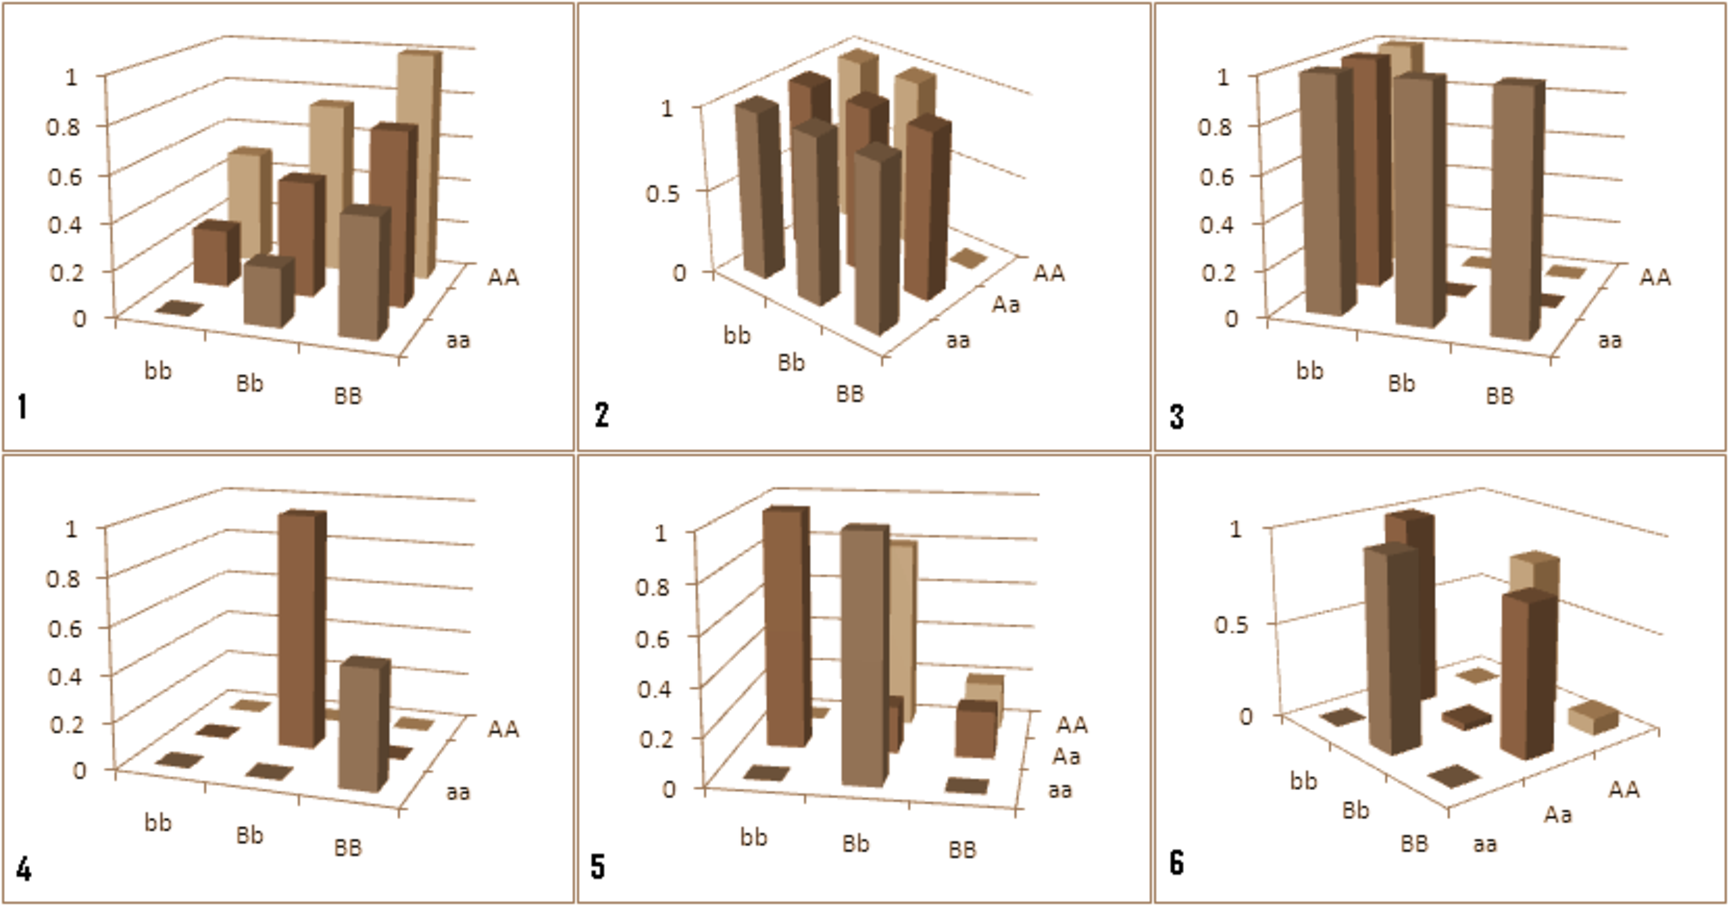
\includegraphics[scale=0.47]{Chapter1/gpmaps2.pdf}
\caption[Genotype phenotype maps]{Genotype-Phenotype maps. 1. Independent additive effects at locus A and B; 2. Dominant pattern of canalisation; 3. Recessive pattern of canalisation; 4-6. Patterns generated by a genetic algorithm optimising for maximised additive variance and long-term survival at intermediate frequency.}
\label{fig:gpmaps}
\end{center}
\end{figure}

Two observations influenced the optimisation strategy used to identify potential genotype-phenotype maps. Firstly, it is assumed that the plausibility and opportunity of the occurrence of independent additive effects is relatively high, for example the actions of many genes are dosage dependent and this prescribes an additive mutation model for their regulation mechanisms \citep{Hedrich2001}. Conversely, while the biological feasibility of some epistatic patterns is fairly high, such as patterns 2 and 3 in figure \ref{fig:gpmaps}, for which numerous molecular examples exist \citep{Nowak1997,Kafri2009,Li2010}, most arrangements of genotype-phenotype maps will not easily describe current observations of variation. Although this could be ascribed to an incomplete understanding of molecular biology, in general the occurrence of epistasis can be said to be rare relative to independent mutational effects. Thus for epistasis to form a significant contribution toward genetic variance it must compensate by persisting over a relatively long period of time, allowing many rare mutation events to accumulate. Secondly, because $h^2$ estimates are relatively constant for traits associated with fitness \citep{Mousseau1987,Bradshaw1991}, it can be hypothesised that evolutionarily persistent epistatic patterns may sustain some additive genetic effects at frequencies that are stable under selection. Using a genetic algorithm to heuristically search the large parameter space of a genotype-phenotype map, a cohort of patterns were generated that locally maximise these conditions, and the three cases that maintained the highest proportion of additive variance (Figure \ref{fig:gpmaps} patterns 4-6) are examined here. While it is difficult to generalise the behaviour of all possible two-locus genotype-phenotype maps, an examination of the potential impact of epistasis from six genotype-phenotype maps was made deterministically and using population simulations, with the same analysis performed on an extended range of maps in the appendix \citep{Li2000}.

Two important results were obtained from the genetic algorithm simulations. First, a diverse range of two-locus genotype-phenotype maps can sustain genetic variance under balancing selection. The significance of this is that while spontaneous occurrence of epistasis may be relatively rare, a reasonable proportion of the two-locus parameter space could effectively mask genetic variance from selection. Furthermore, many of the theoretical models of epistasis under selection discussed previously depend on multi-locus ($>2$) systems to temper the erosion of variance, but by extending parameterisations beyond solely additive-by-additive effects this assumption can be relaxed. Second, the vast majority of this variance is non-additive. While additive variance may be generated at some frequencies, the frequencies that are evolutionarily stable tend to reduce additive variance substantially, relative to the total genetic variance.


\subsection{Allele frequencies under selection}

To assess the potential of epistatic loci maintaining genetic variance at intermediate allele frequencies, thus fulfilling the criterion of the common disease-common variant hypothesis, we analysed the trajectory of the expected allele frequencies under selection over the period of 200 generations (figure \ref{fig:allelefreq}). Twenty-five deterministic simulations (figure \ref{fig:allelefreq_det}) were performed with different initial allele frequencies at both loci, such that all two-locus combinations of the frequencies 0.1, 0.3, 0.5, 0.7 and 0.9 were enumerated. Purely additive effects (pattern 1) are purged rapidly as expected, but in contrast epistatic patterns generally persist over a sustained period (see also figures \ref{fig:sup_allelefreq_det} and \ref{fig:sup_allelefreq_sim}). In particular, patterns 4-6 stabilise at intermediate frequencies.

To accommodate the effects of random drift and incomplete penetrance, further analyses were performed by observing the allele frequencies of the causal loci in simulated populations of 1000 individuals under selection for the same length of time where the genetic variance of the causal loci at generation 0 was 10\% of the total phenotypic variance. The simulations were repeated 50 times with the initial allele frequency set to 0.5 at both loci. A crucial effect of drift is that allele frequency paths can depart from deterministic trajectories, allowing for epistatic variation to persist at intermediate frequencies, even when deleterious effects are large. Here epistasis appears necessary to fulfil the common disease-common variant paradigm. 

Another important consequence is that the perceived rarity of occurrence of epistatic polymorphisms is offset by the inability of selection to purge them from the population, supporting the notion that epistasis could be relatively abundant should such interactions have accumulated over long time periods. In addition, in the context of mutation-selection balance models, since deleterious mutations are fixed slowly for many genotype-phenotype maps, the dependence on a high mutation rate and a highly polygenic architecture to maintain genetic variance is reduced \citep{Phillips2007}.

\begin{figure}
\begin{center}
\subfigure[Deterministic]{\label{fig:allelefreq_det}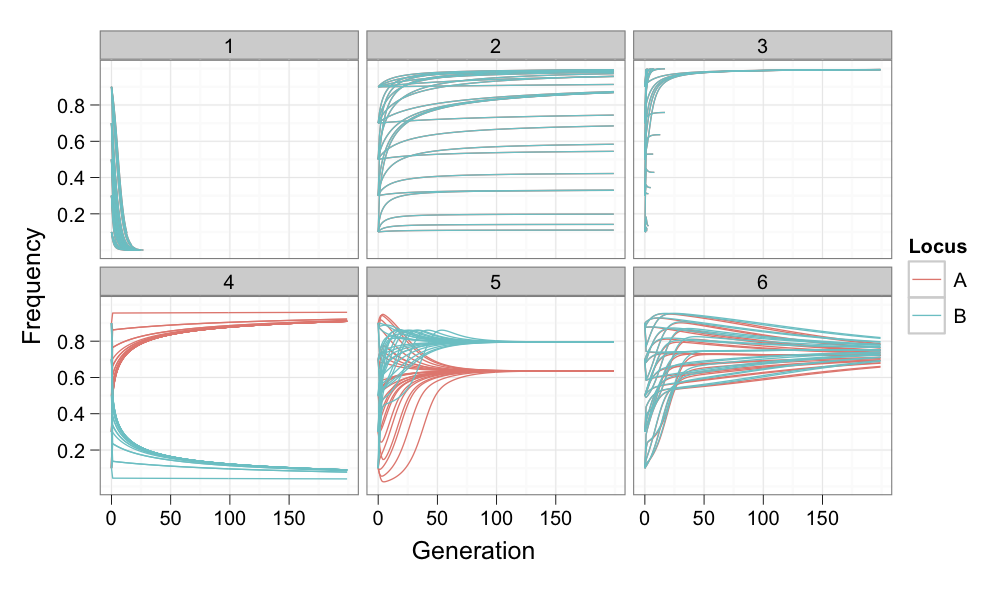
\includegraphics[scale=0.7]{Chapter1/allelefreq_det.png}} \\
\subfigure[Simulated]{\label{fig:allelefreq_sim}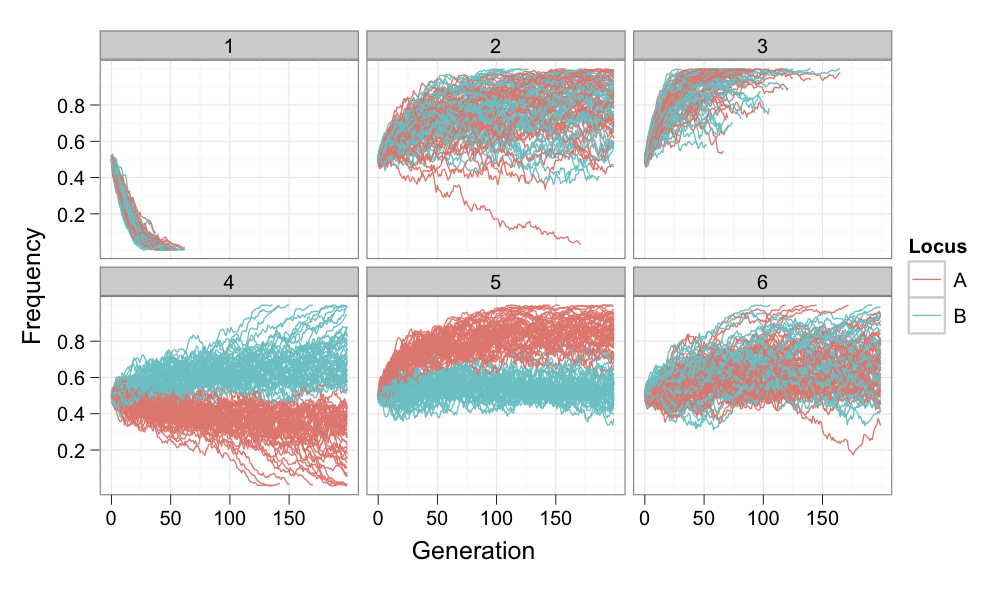
\includegraphics[scale=0.7]{Chapter1/allelefreq_sim.png}} \\
\caption[Allele frequency trajectories for epistasis under selection]{Allele frequencies for two-locus genotype-phenotype maps. \emph{(a)} The expected trajectory of allele frequencies for epistatic fitness patterns (figure \ref{fig:gpmaps}) with initial frequencies of 0.1, 0.3, 0.5, 0.7 and 0.9 enumerated over both loci. \emph{(b)} The path of allele frequencies in simulated populations comprising 1000 individuals and $H^2=10\%$ at generation 0. Boxes represent the different genotype-phenotype maps from figure \ref{fig:gpmaps}.}
\label{fig:allelefreq}
\end{center}
\end{figure}

\subsection{Quantifying additive variance}

The effect of selection on the variance generated by these interactions over time was examined deterministically (figure \ref{fig:var_det}). For those genotype-phenotype maps that reach a stable equilibrium (patterns 4-6) genetic variance is sustained at high levels (figure \ref{fig:Vg_det}), and these types of interactions could be one mechanism by which many fitness traits in experimental situations fail to respond to selection through balancing selection \citep{Hansen2004}. Also considered was the additive variance precipitated by these interactions. As a component of the total genetic variance, the relative magnitude of additive variance is prone to large fluctuations. At some frequencies, particularly early generations or as frequencies approach fixation, most of the variance is expected to be additive, but as the frequencies approach equilibrium the additive variance is mostly lost. Given that one of the optimisation criteria for genotype-phenotype maps generated by the genetic algorithm (patterns 4-6) was to maximise additive variance we can infer that the majority of two-locus epistatic patterns that persist at high intermediate allele frequencies through balancing selection are unlikely to contribute significantly to $h^2$ in fitness traits.

\begin{figure}
\begin{center}
\subfigure[Genetic variance]{\label{fig:Vg_det}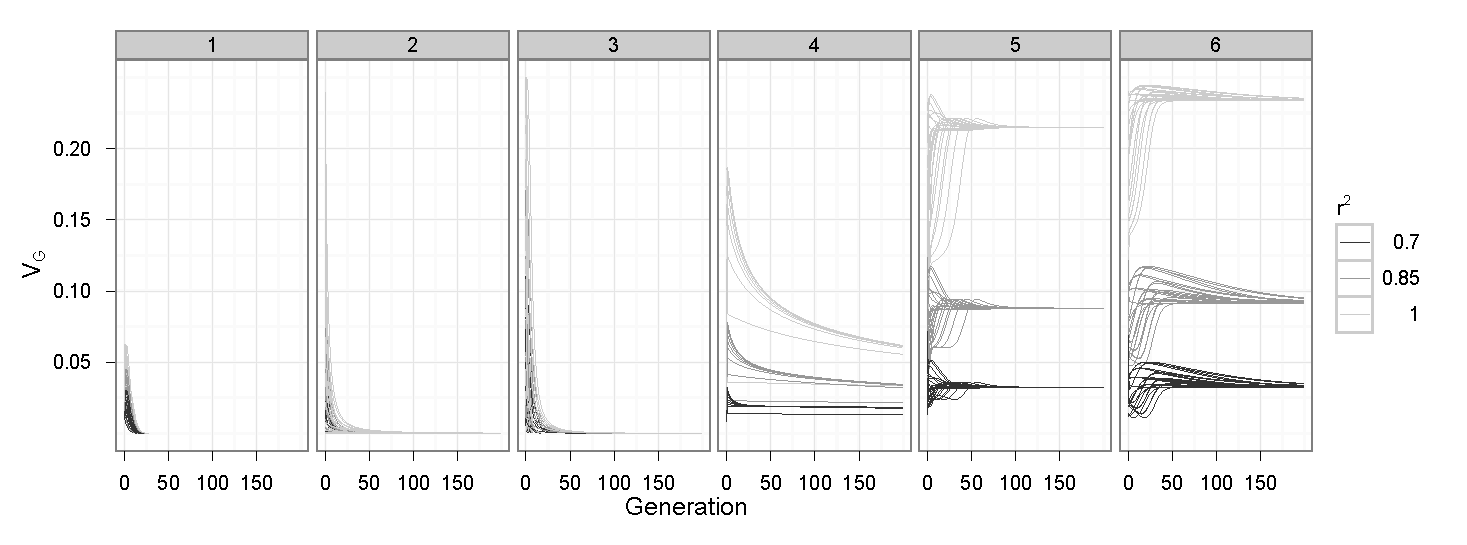
\includegraphics[scale=0.6]{Chapter1/Vg_det_grey.pdf}} \\
\subfigure[Additive variance as a proportion of genetic variance]{\label{fig:propadditive_det}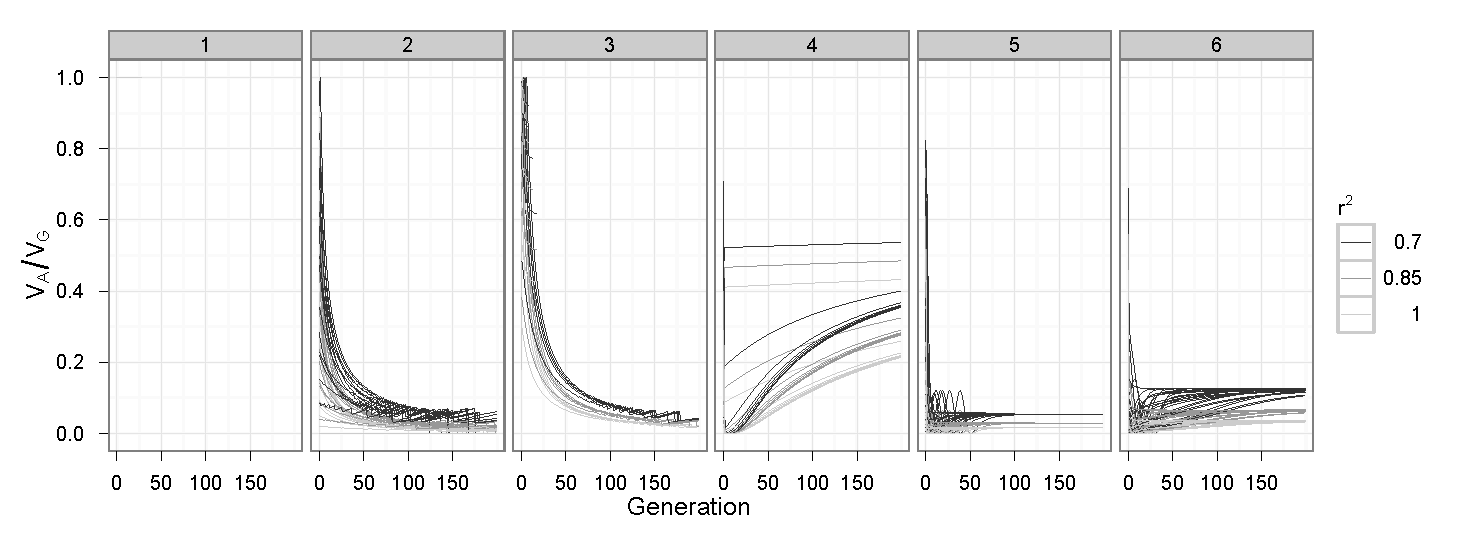
\includegraphics[scale=0.6]{Chapter1/propadditive_det_grey.pdf}} \\
\caption[Deterministic change in variance components]{Deterministic change in variance components of genotype-phenotype maps under selection, with initial frequencies of 0.1, 0.3, 0.5, 0.7 and 0.9 enumerated over both loci. The variance decomposition was performed at the causal locus ($r^{2}=1$), and at SNP pairs that were in incomplete LD with the causal loci. Boxes represent the different genotype-phenotype maps from figure \ref{fig:gpmaps}.}
\label{fig:var_det}
\end{center}
\end{figure}

It is also observed that if the variance of the causal variants is being estimated through incomplete linkage disequilibrium (LD) with neighbouring SNPs, then variance estimates are strongly affected. Not only do the estimates of genetic variance drop rapidly with decreasing LD, but the proportion of the remaining estimated variance that appears additive increases (figure \ref{fig:propadditive_det}). Most association studies parameterise for additive effects, and this may be beneficial for improving detectability, but conclusions about the underlying architecture of these traits may be premature.

In light of this, the performances of different association strategies in identifying the additive variance associated with each of the genotype-phenotype maps under different conditions of linkage disequilibrium were compared (figure \ref{fig:heritability}). Also compared was the power of one dimensional analyses, typical of GWASs, against two dimensional analyses where each SNP is tested for interaction with all other SNPs. Here, the power is defined as the proportion of the total additive variance across the populations that is explained. For the one dimensional scans p-values were calculated from linear regression analyses parameterised for purely additive effects, as is routine for GWASs, or full genotype effects (additive + dominance). These were tested for significance by applying a Bonferroni threshold assuming a multiple testing penalty incurred by using a 300k SNP chip ($1.7\times10^{-6}$) at the 5\% family-wise significance level. Two dimensional scans were performed in a similar vein, the tests being parameterised in three ways (additive and dominance effects at both loci, only interaction terms, or all terms), and a Bonferroni testing threshold imposed ($1.1\times10^{-11}$).

With the goal of detecting variants comprising $h^2$, it is intuitive to perform association scans using an additive model, but perhaps other parameterisations would be more suitable if the persistence of additive variation was maintained by a more complicated genetic architecture. Several testing parameterisations were compared for their power to explain the additive variance of the genotype-phenotype map. For one dimensional scans additive models were compared against the 2 degree of freedom additive + dominance effects, and for two dimensional scans the efficacy of looking for solely marginal effects (4 degrees of freedom), solely interaction terms (4 degrees of freedom) \citep{Cordell2002}, or the full two locus genetic effect (8 degrees of freedom) were compared.

There are two immediately noticeable results from these analyses. First, there is no single approach that generally performs the best in all situations (figures \ref{fig:heritbars_det} and \ref{fig:sup_heritbars_det}). Second, it is clear that parameterising the test as an additive model is rarely the most powerful approach. Of the 55 non-neutral patterns in figure \ref{fig:sup_gpmaps}, when LD between causal variants and observed SNPs is high the two dimensional full genetic test is most powerful for 44 of them. This performance decays rapidly with reduced LD, to being most powerful only 3 times at $r^2=0.7$. Instead, at lower LD, parameterising for additive + dominance in one dimension is most powerful for 36 of the patterns. The marginal and interaction parameterisations of the two dimensional scans were seldom as powerful as the full genetic test.

A more detailed recording of the change in power over time under selection is shown in figure \ref{fig:heritability_sim}. Of total additive variance summed across all simulated populations, the fluctuations of the proportion detectable by the two most powerful methods, full genetic in one dimension and full genetic in two dimensions, is tracked. While patterns 2 and 3, examples of canalisation, do persist for relatively prolonged periods, the majority of this time is spent at low frequencies such that insufficient variance is generated to be detectable. When limited to the two-locus case, canalisation may be less important at maintaining phenotypic variation than has been suggested in other studies based on multiple loci (\emph{e.g.} \citealp{Carter2005}).

The results of the power comparison between patterns 4-6 in figure \ref{fig:heritability_sim} can be explained logically to some extent from the results in figures \ref{fig:propadditive_det} and \ref{fig:rsq_v_vg}. The first problem encountered by the two dimensional test is that as LD between causal variants and observed SNPs is reduced there is a dramatic decline in the total genetic variance, this is irreconcilable with a heavy multiple testing penalty. The second problem is that the remaining genetic variance is increasingly heavily represented by additive variance as the LD drops (as demonstrated in figure \ref{fig:rsq_v_vg}), such that the trade off between variance explained and the number of degrees of freedom becomes detrimental. The converse is true for the one dimensional test, where the exclusion of higher order variance components loses relevance.


\begin{figure}
\begin{center}
\subfigure[Deterministic patterns of $V_A$ detection]{\label{fig:heritbars_det}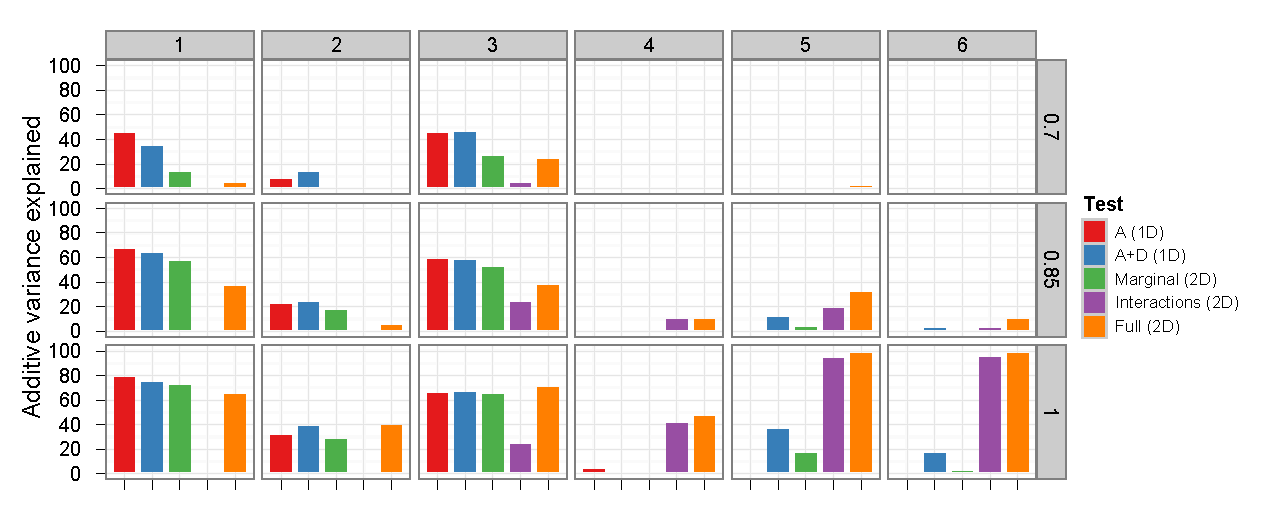
\includegraphics[scale=0.73]{Chapter1/heritbars_det.pdf}} \\
\subfigure[$V_A$ detected through simulation]{\label{fig:heritability_sim}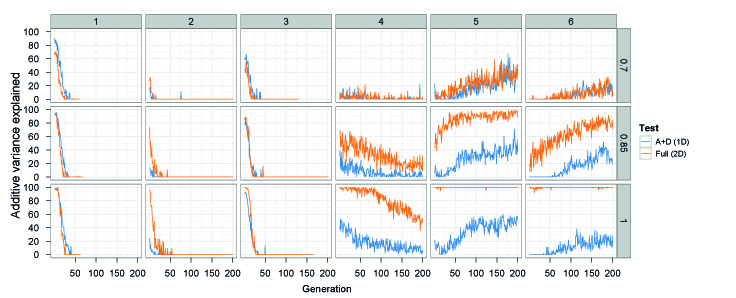
\includegraphics[scale=0.6]{Chapter1/heritability_sim.jpg}} \\
%\subfigure[Overall performance comparison of testing strategies during simulations]{\label{fig:heritbars_sim}\includegraphics[scale=0.4]{Chapter1/heritbars_sim.pdf}}
\caption[Proportion of additive variance detected]{The percentage of total additive variance detected by each of 5 different methods. Columns of graphs refer to genotype-phenotype maps (figure \ref{fig:gpmaps}), rows refer to $r^{2}$ between causal variants and observed SNPs. \emph{(a)} Deterministic calculations were performed 25 times, each with different initial allele frequencies. The percentage of additive variance explained is summed across all runs and generations. \emph{(b)} The summed $V_A$ detected at each generation as a percentage of the summed $V_A$ simultaneously present in 50 populations. For clarity, only the most powerful 1D test (A+D) is compared against the most powerful 2D test (full parameterisation).}
\label{fig:heritability}
\end{center}
\end{figure}

\section{Discussion}

While some studies have pointed out the failings of genome wide association studies, and thrown doubt upon the common disease-common variant paradigm, several others have nominated epistasis as a potential mechanism to reconcile these problems, and as a source of the `missing heritability'  \citep{Manolio2009,Frazer2009}. This study sought to investigate these claims in the context of two-locus functional epistasis in traits under selection.

Initially it was investigated whether or not deleterious mutations could be maintained as common polymorphisms. By assaying a large sample of potential genotype-phenotype maps \citep{Li2000}, and artificially selecting for new maps using a genetic algorithm, it was demonstrated that a substantial improvement in the maintenance of genetic variance at intermediate frequencies could be made compared to independent additive effects (figures \ref{fig:sup_allelefreq_det} and \ref{fig:sup_allelefreq_sim}). This finding is in agreement with theories of balancing selection \citep{Hansen2004}, and the potential for epistatic interactions between polymorphisms is increased under fitness related traits because of their more polygenic architecture \citep{Lande1975}.

Following on, the potential for these interactions to maintain additive genetic variance was explored. It was clearly demonstrated that even in the best case scenario, where genotype-phenotype maps were generated to maximise additive variance, total genetic variance was mostly composed of non-additive components (figures \ref{fig:propadditive_det} and \ref{fig:sup_propadditive_det}). This finding is in disagreement with a recent study \citep{Hill2008a}, which showed that for various two-locus epistatic models, the deterministic partitions of genetic variance calculated across different frequency distributions were largely dominated by the additive component. This study finds that those allele frequencies at which additive variance is high (a large proportion of the frequency spectrum), are evolutionarily unlikely, thus should epistatic variants be affecting fitness traits it is reasonable to believe that the majority of the variance will be non-additive. Ultimately there is no simple mechanism whereby two-locus epistasis will significantly contribute toward the missing heritability, unless $h^2$ estimates have been contaminated by non-additive components (\emph{e.g.} full-sib based estimates).

Another observation regarding the perceived contribution of additive variance can also be made. When partitioning the variance components of the genotype-phenotype maps through the proxy of markers in incomplete linkage disequilibrium with the true causal variants, there is a danger of overestimating the relative contributions of additive to non-additive variance. \cite{Weir2008} shows that the decay in additive variance is linear with decreasing $r^2$ but quadratic for dominance variance. For more complex genotype-phenotype maps that include higher order variance components it is more complicated (figure \ref{fig:rsq_v_vg}), but in general the decay of non-additive variance is much more rapid than additive. Resultantly, those markers that are detected in GWAS may appear more additive than the dominant or epistatic causal variants with which they are associated.

\begin{figure}
\begin{center}
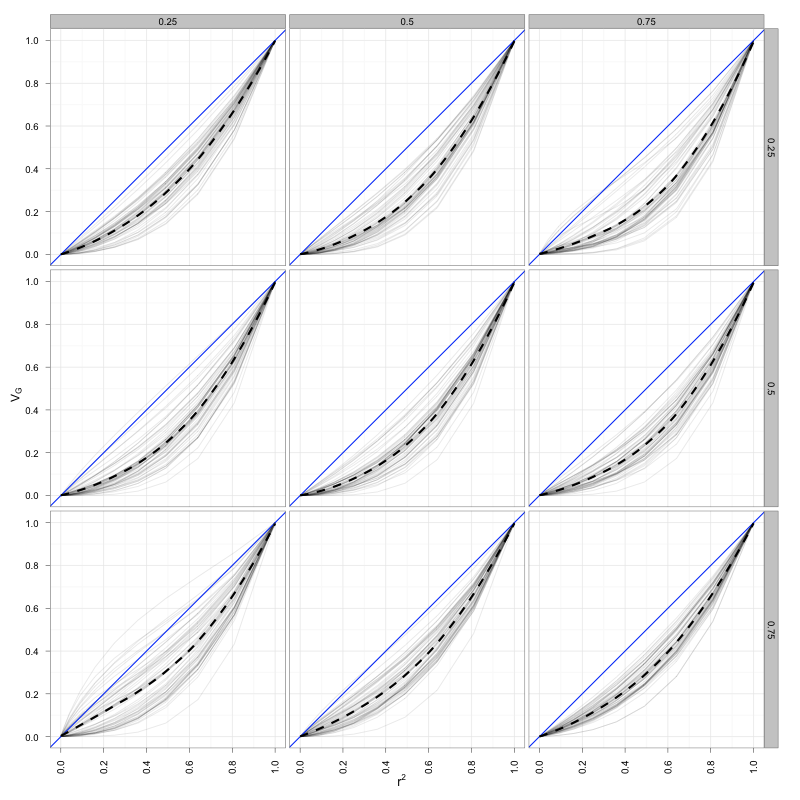
\includegraphics[scale=0.4]{Chapter1/rsq_v_vg.png} \\
\caption[Epistatic variance estimates as a function of LD]{Relationship between genetic variance of observed SNPs (y axis) and their linkage disequilibrium with causal variants (x axis). Observed SNPs have the same allele frequency as their linked causal variants, and there is no linkage disequilibrium between causal variants or between observed SNPs. Blue line represents a purely additive genotype-phenotype map, faint black lines each represent the 55 dominant or epistatic genotype-phenotype maps in figure \ref{fig:sup_gpmaps}, and the black dashed line represents the smoothed average of all black lines. Allele frequencies of genotype-phenotype maps are represented by boxes, the frequency of locus A horizontally and locus B vertically.}
\label{fig:rsq_v_vg}
\end{center}
\end{figure}


The simulations suggest that we should expect significant levels of non-additive variance in fitness traits. While non-additive variances are often considered to be nuisance terms in quantitative genetics, perhaps their existence, the variance lurking beneath the surface, can be levered to actually improve the detection of additive variance whilst also acquiring knowledge of the non-additive components. Power comparisons were made between one and two dimensional scans, as well as different testing parameterisations, with a view to detecting variants under selection at evolutionarily likely frequencies. Surprisingly, the simplest and most widely used parameterisation, modelling for additive effects in one dimension, was seldom the most powerful approach. On the contrary, because other forms of genetic variance are co-precipitated along with additive variance, by parameterising the tests to include them the power was seen to improve. However, it was observed that even with modest reductions in LD between causal variants and observed SNPs all testing strategies tended to decline in performance rapidly. This leaves researchers in a difficult situation, where the strategy of increasing SNP panel densities as an intuitive response to improve LD coverage comes at a quadratic cost (in the two-locus case) in computation time and multiple testing penalties.

Nevertheless, some optimism can be derived from the observation that many genotype-phenotype maps are capable of sustaining common variants for relatively prolonged time scales, and various strategies can be employed to improve the power of their detection. For example, in order to improve the power of one dimensional scans, it appears expedient to increase the parameterisation to two degrees of freedom by including dominance (figures \ref{fig:heritbars_det} and \ref{fig:sup_heritbars_det}). It may also be worth considering the use of multiple-marker methods, such as haplotype associations, as a means to curtail the loss of information through insufficient LD \citep{Schaid2004}. Further, the multiple testing penalties here assume a family of independent tests, however given the correlation structure within a SNP panel the effective number of tests is likely to be lower \citep{Dudbridge2008}. How much lower when the search is expanded to two dimensions is unknown, but if taken into consideration this could significantly improve the performance.

Although the intention behind the genetic algorithm was to explore the potential for a two-locus system to maintain additive variance, rather than to necessarily identify biologically feasible maps, those maps that emerged did not appear biologically untenable. In fact they can be supported by reports in the literature due to their tendencies for exhibiting heterozygote advantage \citep{Comings2000, Luo2001}. The example of the single locus case, overdominance, is central to processes of heterosis and inbreeding depression \citep{Moll1965, Luo2001}, and has been identified in molecular studies also \citep{Chen1994, Miskimins1986}. Indeed, heterozygote advantage plays an important role in evolutionary theory, as it confers segregational load on a population, and this type of load cannot be purged due to balancing selection, potentially rendering populations susceptible to accumulating a critical mass of such polymorphisms \citep{Dobzhansky1970}. The idea of a critical mass of deleterious mutations has been widely explored in amictic haploid populations, particularly in the context of Muller's ratchet, and in this case synergistic epistasis has been suggested as a mechanism that could alleviate the problem in some situations \citep{Kondrashov1994, Butcher1995}. This study may offer a similar answer for the analogous problem of segregational load in diploid populations, because it can be observed that while patterns of overdominance (figure \ref{fig:sup_allelefreq_sim}, pattern 55) form a stable equilibrium, small perturbations to this genotype-phenotype map through the introduction of an interacting locus (\emph{e.g.} patterns 45, 47, 53) could destabilise the equilibrium and lead to eventual fixation.

Much debate has been granted towards the `missing heritability' in complex traits, and while it is an important issue for both understanding genetic systems and moving towards applications in genetic prediction, perhaps the broader problem of the `missing genetic variance' has been unfairly marginalised. On expanding considerations beyond purely additive effects it becomes apparent that while theory suggests an important role for dominance and epistasis for fitness traits \citep{Waddington1942,Kaneko2009,Siegal2002,Gjuvsland2007,Gao2010,Bergman2003,Lane2010}, not only are these types of causal variants seldom searched for, but estimates of these types of variation are seldom being made. Ignoring the higher components of the architecture of complex traits will potentially restrict understanding of these genetic systems and have a detrimental impact on prediction accuracy.


